\documentclass[10pt, aspectratio=169]{beamer}
\usepackage[utf8]{inputenc}
\usepackage[T1]{fontenc}
\usepackage{lmodern}
\usepackage{amsfonts}
\usepackage{amsthm}
\usefonttheme[onlymath]{serif}
\usecolortheme[named=blue]{structure}
\usepackage{graphicx}


\setbeamercolor{block title}{use=structure,fg=white,bg=structure.fg!75!black}
\setbeamercolor{block body}{parent=normal text,use=block title,bg=block title.bg!8!bg}
%\usepackage[scale=5]{beamerposter}

\AtBeginSection[]
{
	\begin{frame}[noframenumbering,plain]
		\frametitle{Outline: Next Topic}
		\tableofcontents[currentsection]
		%		\addtocounter{framenumber}{-1}
	\end{frame}
}

\title{A Formal Approach to Explainability}
\subtitle{(by Lior Wolf, Tomer Galanti, and Tamir Hazan)}
\date{\today}
\author{Phaphontee Yamchote}

\newcommand{\R}{\mathbb{R}}
\newcommand{\N}{\mathbb{N}}

\begin{document}
	\titlepage
	\begin{frame}[noframenumbering,plain]{Outline}
		\tableofcontents
	\end{frame}
	\section{Setting}
	\begin{frame}{Setting}
		Let 
		\begin{itemize}
			\item an input space $\mathcal{X}$
			\item an output space $\mathcal{Y}$ 
			\item a representation space $\mathcal{R}$
			\item an explanation space $G$
			\item a representation function $f:\mathcal{X}\to\mathcal{R}$
			\item a classifier function $c:\mathcal{R}\to\mathcal{Y}$
		\end{itemize}
		
		We want to explain a model $h = c\circ f$\\
		by an explanation function $g:\mathcal{X}\times\mathcal{Y}\to G$\\
		in terms of $g(x,h(x))$
	\end{frame}
	
	\section{Consistency and Explainability of Representation}
	
	\begin{frame}[t]{Representation Space \& Explanation Space}{Consistency}
		\begin{definition}[Consistent Representation]
			Given a function $\beta: (0, \infty)\to (0, \infty)$ mapping distance in $\mathcal{R}$ into distance in $G$.\\
			A representation $f$ is \underline{$\beta$-consistent} w.r.t. $g$ if
			$$
			\forall\epsilon>0\forall x_1, x_2 \in \mathcal{X}, \left|g(x_1, h(x_1)) - g(x_2,h(x_2))\right|\leqslant\epsilon \Rightarrow \left|f(x_1) - f(x_2)\right|\leqslant \beta(\epsilon)
			$$
		\end{definition}
	\end{frame}
	\begin{frame}[t]{Representation Space \& Explanation Space}{Explainability}
		\begin{definition}[Explainable Representation]
			Given a function $\gamma: (0, \infty)\to (0, \infty)$ mapping distance in $\mathcal{R}$ into distance in $G$.\\
			A representation $f$ is \underline{$\gamma$-explainable} w.r.t. $g$ if
			$$
			\forall\epsilon>0\forall x_1, x_2 \in \mathcal{X}, \left|f(x_1) - f(x_2)\right|\leqslant\epsilon \Rightarrow  \left|g(x_1, h(x_1)) - g(x_2,h(x_2))\right|\leqslant\gamma(\epsilon)
			$$
		\end{definition}
		
		\pause\begin{definition}[Second-order Explainable Representation]
			Given a function $\gamma: (0, \infty)\times(0, \infty)\to (0, \infty)$.\\
			A representation $f$ is \underline{second-order $\gamma$-explainable} w.r.t. $g$ if
			$$
			\forall\epsilon_0\epsilon_1>0\forall x_1, x_2 \in \mathcal{X},
			\left|f(x_1) - f(x_2)\right|\leqslant\epsilon_0
			\wedge
			\left|f_x(x_1) - f_x(x_2)\right|\leqslant\epsilon_1$$
			$$
			\Downarrow
			$$
			$$
			\left|g(x_1, h(x_1)) - g(x_2,h(x_2))\right|\leqslant\gamma(\epsilon_0,\epsilon_1)
			$$
		\end{definition}
	\end{frame}
	\begin{frame}[t]{Representation Space \& Explanation Space}{Consistency Recall}
		$$
		\forall\epsilon>0\forall x_1, x_2 \in \mathcal{X}, \left|g(x_1, h(x_1)) - g(x_2,h(x_2))\right|\leqslant\epsilon \Rightarrow \left|\mathcolor{red}{f}(x_1) - \mathcolor{red}{f}(x_2)\right|\leqslant \beta(\epsilon)
		$$
		\begin{itemize}
			\item What if the representation of our machine learning model is consistent, i.e. $h(x)=c(\mathcolor{red}{f}(x))$ where $\mathcolor{red}{f}$ is consistent?
			
			\item Let try: $\left|h(x_1) - h(x_2)\right| = \left|c(f(x_1)) - c(f(x_2))\right|$.
			
			\item What can connect between $\left|c(f(x_1)) - c(f(x_2))\right|$ and $\left|f(x_1) - f(x_2)\right|$?
		\end{itemize}
		
		\begin{definition}[$l$-Lipschitz continuous]
			A function $L$ is $l$-Lipschitz continuous if
			$$
			\forall x_1, x_2, \left|F(x_1)-F(x_2)\right|\leqslant l \left|x_1 - x_2\right|
			$$
		\end{definition}
	\end{frame}
	\begin{frame}[t]{Representation Space \& Explanation Space}{Consistency representation and Lipschitz classifier}
		\begin{theorem}[Lipschitz $\circ$ Consistent is Consistent]
			Given a model $h=c\circ f : \mathcal{X}\to\mathcal{Y}$ with an explanation function $g:\mathcal{X}\times\mathcal{Y}\to G$,\\
			if $f$ is $\beta$-consistent w.r.t. $g$ and $c$ is $l$-Lipschitz continuous,\\
			then $h$ is $l\beta$-consistent w.r.t. $g$.
		\end{theorem}
		Let's prove!
	\end{frame}
	
	\begin{frame}[t]{Representation Space \& Explanation Space}{Explainable representation and Lipschitz classifier}
		$$
		\forall\epsilon>0\forall x_1, x_2 \in \mathcal{X}, \left|f(x_1) - f(x_2)\right|\leqslant\epsilon \Rightarrow  \left|g(x_1, h(x_1)) - g(x_2,h(x_2))\right|\leqslant\gamma(\epsilon)
		$$
		\begin{theorem}[upstream function in Lipschitz $\circ$ Consistent is consistent]
			Given a model $h=c\circ (f_2 \circ f_1) : \mathcal{X}\to\mathcal{Y}$ with an explanation function $g:\mathcal{X}\times\mathcal{Y}\to G$,\\
			if $f$ is $\gamma$-explainable w.r.t. $g$ and $c$ is $l$-Lipschitz continuous,\\
			then $f_1$ is $\hat{\gamma}$-explainable w.r.t. $g$ where $\hat{\gamma}(\epsilon):=\gamma(l\epsilon)$.
		\end{theorem}
	\end{frame}
	
	\begin{frame}{Case Study: Image Classification}
		\begin{center}
			I still don't understand this topic right now,\\ it requires background in image processing, which I'm not familiar with
		\end{center}
		% TODO: \usepackage{graphicx} required
		\begin{figure}
			\centering
			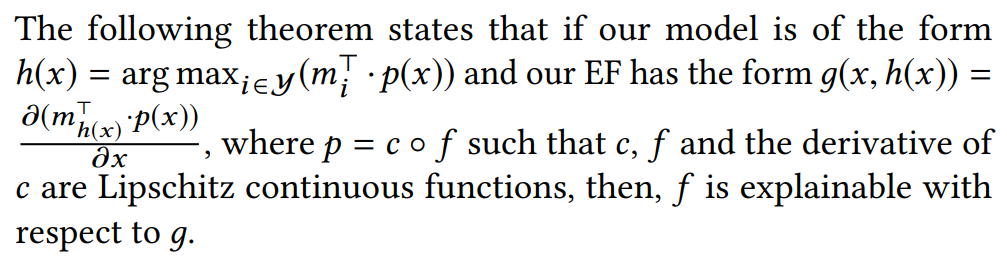
\includegraphics[width=0.7\linewidth]{screenshot001}
			\centering
			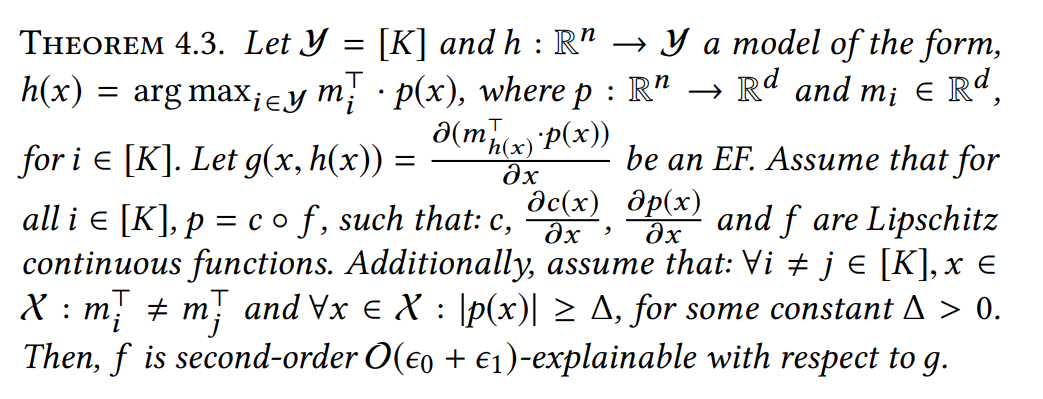
\includegraphics[width=0.7\linewidth]{screenshot002}
		\end{figure}
		
	\end{frame}
	
	\section{Validity and Completeness of Explanation Function}
	
	\begin{frame}[t]{Properties of Explanation Functions}{Validity}
		\begin{definition}[Valid Explanation Functions]
			Given a fixed constant $\epsilon>0$ and $x\sim \mathcal{D}$.\\
			An explanation function $g$ is \underline{$\epsilon$-valid} w.r.t. a model $h$\\
			if there is a function $t:G\to\mathcal{Y}$ s.t.
			$$
			\mathbb{E}_{x\sim\mathcal{D}}\left[ \ell\left(t\left(g\left(x,h\left(x\right)\right)\right),h\left(x\right)\right) \right]\leqslant\epsilon,
			$$
			where $\ell$ is a loss function.
		\end{definition}
	\end{frame}
	
	\begin{frame}[t]{Properties of Explanation Functions}{Completeness}
		\begin{definition}[Complete Explanation Functions]
			Given a fixed constant $\alpha,\epsilon>0$ and $x\sim \mathcal{D}$.\\
			An explanation function $g$ is \underline{$(\epsilon,\alpha)$-complete} w.r.t. a model $h$\\
			if every $\bar{g}:\mathcal{X}\to\R^d$ s.t. $I(g(x,h(x));\bar{g}(x))\leqslant\epsilon$ and every $s:\R^d\to\mathcal{Y}$
			$$
				\mathbb{E}_{x\sim\mathcal{D}}\left[ \ell
					\left(
						s(\bar{g}(x)), h(x)
					\right)
				\right]\geqslant\alpha,
			$$
			
			where $\ell$ is a loss function.
		\end{definition}
	\end{frame}
	
	\begin{frame}{Properties of Explanation Functions}
		if we are able to recover $h(x)$ from $\bar{g}(x)$ and from $g(x, h(x))$, then, $\bar{g}(x)$ and $g(x, h(x))$ cannot be independent of each other.
		\begin{theorem}[Valid $\Rightarrow$ Complete]
			Let $h: \mathbb{R}^n \rightarrow \mathcal{Y}$ be a model, $g: \mathcal{Z} \rightarrow G$ an $\epsilon_0$-valid EF for some constant $\epsilon_0 \in(0,0.5)$ and $x \sim D$.\\
			Assume that $Y=\{ \pm 1\}$ and denote, $p:=\mathbb{P}[h(x)=1]$.\\
			Then, $g$ is $(\epsilon, \alpha)$-complete with respect to $h$, with $\alpha:=\frac{\sqrt{1+H(p)\left(H(p)-\epsilon-2 \sqrt{\epsilon_0}\right)}-1}{H(p)}$ and any $\epsilon>0$ that satisfies, $H(p)>\epsilon+2 \sqrt{\epsilon_0}$.\\
			In particular, if $p=1 / 2$, we have: $\alpha=\sqrt{2-\epsilon-2 \sqrt{\epsilon_0}}-1$.
		\end{theorem}
		Need a lot of lemmas from other works
	\end{frame}
	
	
	\section{Arithmetic of Explanations}

	\begin{frame}{Intersection and Union of RVs}
		\begin{definition}
			Let $x\sim\mathcal{D}$ on $\mathcal{X}$, a constant $\epsilon>0$ and\\
			given two functions $f_1:\mathcal{X}\to\mathcal{X}_1$ and $f_2:\mathcal{X}\to\mathcal{X}_2$.\\
			If there are two invertible functions $r_1:\mathcal{X}_1\to\mathcal{V}_1$ and $r_2:\mathcal{X}_2\to\mathcal{V}_2$
			such that
			\begin{align*}
				r_1(f_1(x)) &= (e_1(x),u(x))\\
				r_2(f_2(x)) &= (e_2(x),u(x)),
			\end{align*}
			where mutual information $I(e_i(x);f_j(x))\leqslant\epsilon$ for $i\neq j\in\{1,2\}$
			\begin{itemize}
				\item the RV $u(x)$ is called \underline{$\epsilon$-intersection} of $f_1$ and $f_2$
				\item the RV $(e_1(x), u(x), e_2(x))$ is \underline{$\epsilon$-union} of $f_1$ and $f_2$
			\end{itemize}
		\end{definition}
		(Still don't get its idea why define like this)\\
		(this work as well proved that they are unique up to invertible transformation)
	\end{frame}
	
\end{document}